%% Template for ENG 401 reports
%% by Robin Turner
%% Adapted from the IEEE peer review template

%
% note that the "draftcls" or "draftclsnofoot", not "draft", option
% should be used if it is desired that the figures are to be displayed in
% draft mode.

\documentclass{article}
\usepackage{url} % Provides better formatting of URLs.
\usepackage[utf8]{inputenc} % Allows Spanish characters.
\usepackage[spanish]{babel}
\usepackage{amssymb}
\usepackage{booktabs} % Allows the use of \toprule, \midrule and \bottomrule in tables for horizontal lines
\usepackage{float}
\usepackage{pdfpages}
\usepackage{graphicx}
\usepackage{booktabs}
\usepackage{fancyhdr}
\usepackage{eurosym}
\usepackage{calendar}



\hyphenation{op-tical net-works semi-conduc-tor} % Corrects some bad hyphenation 



\begin{document}
%\begin{titlepage}
% paper title
% can use linebreaks \\ within to get better formatting as desired
\title{
\includegraphics[scale=0.65]{logoDefinitivo1.png} \\ \textbf{Proyecto UPBEAT} \\ \textbf{Grupo 03. Barbara Liskov}\\Plan de gestión, análisis y memoria del proyecto \vspace{0.1cm} \\}

% author names and affiliations

\author{Alejandro Ruiz Sumelzo\\
Alejandro Piedrafita Barrantes\\
Álvaro Santamaría De la Fuente\\
Fernando Navarro Zarralanga\\
José Félix Yagüe Royo\\
Víctor Pérez Sanmartín\\
Sergio Torres Castillo \vspace{0.25cm}
\\\\

\includegraphics[scale=0.5]{logoUZ.png}\\
}
\date{8 de junio de 2020}

% make the title area
\maketitle
\newpage
\section*{Introducción}
El proyecto \textit{Upbeat} consiste en el desarrollo e implementación de un reproductor de música en streaming.\\
\hfill \break
La aplicación está diseñada para todo tipo de público, incluidos artistas. Permitirá a los usuarios escuchar canciones o podcasts, crear listas de reproducción, añadir canciones o podcasts a su lista de favoritos para después acceder a sus contenidos preferidos de una forma más rápida o seguir a otros usuarios entre otras funcionalidades.
\hfill \break\\
De manera similar, los artistas tendrán las mismas características que cualquier usuario además de poder subir canciones y/o crear álbumes. Esto será algo exclusivo de las cuentas de clientes registradas como artistas.
\hfill \break
Añadirá aspectos de la 'red social', tales como seguir a otros usuarios o sus playlist creadas.\\
\hfill \break
Otras de las características diferenciales de nuestra aplicación será el uso de banners de publicidad o la implementación de un ecualizador de sonido que modificará la manera de reproducir las canciones.\\\\
Por último, el reproductor de música \textit{Upbeat} permitirá realizar una búsqueda por título de canción, género, artista y país de la misma.\\\\
Se permitirá usar la aplicación de tres maneras diferentes: Mediante una aplicación web (navegador Chrome), una aplicación para dispositivos\textit{Android} y una aplicación para dispositivos \textit{iOS}.\\\\
Las 3 versiones de la aplicación serán muy similares, salvo que un pequeño número de características solo estarán disponibles en la versión web, como el ecualizador de sonido o los banners de publicidad. \\\\
Usará también un sistema de sincronización, permitiendo que el usuario retome cualquier canción donde la había dejado, en todos los dispositivos.


\newpage
\tableofcontents % si estas líneas se comentan, se eliminan los índices
%\listoffigures
%\listoftables
\addtocontents{toc}{\hfill \textbf{Página} \par}
\newpage
\pagestyle{fancy}
\lhead{\begin{picture}(0,0) \put(0,0){\includegraphics[width=40mm]{logoEina.png}} \end{picture}}
\rhead{\begin{picture}(0,0) \put(-100.7,0){
\includegraphics[width=35mm]{logoDefinitivo3.png}} \end{picture}}
\section{Organización del proyecto}
\begin{table}[H]
	\hspace*{-3.7cm}
	\centering
	\begin{tabular}{|l|l|l|}
		\hline
		\multicolumn{1}{|c|}{\textbf{Integrante}} & \multicolumn{1}{c|}{\textbf{Puesto}} & \multicolumn{1}{c|}{\textbf{Responsabilidades}}\\ \hline
		Alejandro Ruiz Sumelzo                    & \begin{tabular}[c]{@{}l@{}}Director del proyecto.\\ Coordinador y desarrollador del grupo de back-end.\\ Encargado de la documentación del análisis y diseño\\ del sistema.\end{tabular} & \begin{tabular}[c]{@{}l@{}}Responsable de redactar algunas actas\\ en reuniones con el profesor.\\ Control de la distribución de trabajo\\ (elaboración de calendario) y \\ revisión de esfuerzos.\\ Desarrollador de modelos, repositorios y \\controladores de la API.\\ Encargado del despliegue del back end \\sobre el servidor.\end{tabular} \\ \hline
		\begin{tabular}[c]{@{}c@{}}Alejandro\\ Piedrafita Barrantes\end{tabular}
		&                                                                       Desarrollador de apoyo para el grupo de back-end                                                                                                                 &  
		\begin{tabular}[c]{@{}l@{}}Realización de tareas de gestión\\  (edición de memoria y otros documentos).\\ Desarrollador de modelos, repositorios y \\ controladores de la API. \\ Diseño del sistema mediante diagramas.\end{tabular}\\ \hline
		\begin{tabular}[c]{@{}c@{}}Víctor\\ Pérez Sanmartín\end{tabular}
		&                                                                       Desarrollador de apoyo para el grupo de back-end                                                                                                                 &  
		\begin{tabular}[c]{@{}l@{}}
		Responsable de redactar algunas actas\\ en reuniones con el profesor.\\
		Realización de tareas de gestión\\  (edición de memoria y otros documentos).\\ Desarrollador de modelos, repositorios y \\ controladores de la API. \\ Encargado del diseño e implementación\\ de la base de datos.\end{tabular}\\ \hline
		\begin{tabular}[c]{@{}c@{}}Álvaro Santamaría\\ de la Fuente\end{tabular}
		& \begin{tabular}[c]{@{}l@{}}  Desarrollador del grupo de front-end móvil.\end{tabular}     &  
		\begin{tabular}[c]{@{}l@{}}
		Realización de tareas de gestión\\ (edición de memoria y otros documentos).\\
		Desarrollo e implementación del front-end \\de la aplicación móvil.\\
		Implementar la lógica de la aplicación de\\ \textit{Android} e \textit{iOS}.\\
		Encargado de unificar las partes \\de la aplicación móvil y llevar a cabo \\ el despliegue en \textit{Android} e \textit{iOS}.
		\end{tabular}\\ \hline
		\begin{tabular}[c]{@{}c@{}}José Félix Yagüe\\ Royo\end{tabular}
		&                                                                       \begin{tabular}[c]{@{}l@{}}  Desarrollador del grupo de front-end móvil.\\ Encargado de la gestión de la parte front móvil \\ del proyecto.\end{tabular}                                                  &  
		\begin{tabular}[c]{@{}l@{}}Realización de tareas de gestión\\ (edición de memoria y otros documentos).\\
		Desarrollo e implementación del front end \\de la aplicación móvil.\\
		Encargado de la conexión con el API REST. \\
		Control de la distribución de trabajo y \\ coordinación dentro del grupo \\ front-end de móvil.\\\end{tabular}\\ \hline
	\end{tabular}
\end{table}

\begin{table}[H]
	\hspace*{-3.7cm}
	\centering
	\begin{tabular}{|l|l|l|}
		\hline
		\multicolumn{1}{|c|}{\textbf{Integrante}} & \multicolumn{1}{c|}{\textbf{Puesto}} & \multicolumn{1}{c|}{\textbf{Responsabilidades}}\\ \hline
		\begin{tabular}[c]{@{}c@{}}Fernando\\ Navarro Zarralanga\end{tabular}           
		& 
		\begin{tabular}[c]{@{}l@{}}Coordinador y desarrollador del grupo de \\ front-end web.\\ Encargado de la gestión de la parte front web \\ del proyecto.\end{tabular} & \begin{tabular}[c]{@{}l@{}}Realización de tareas de gestión\\ (edición de memoria y otros documentos).\\ Diseñar pantallas de la aplicación de la web.\\
		Implementar la lógica de la \\ aplicación web.\\ 
		Encargado de llevar a cabo el despliegue \\de la web.
		\end{tabular} \\ \hline
		\begin{tabular}[c]{@{}c@{}}Sergio\\ Torres Castillo\end{tabular}
		&                                                                       Desarrollador de apoyo para el grupo de front-end                                                                                                                 &  
		\begin{tabular}[c]{@{}l@{}}
			Realización de tareas de gestión\\ (edición de memoria y otros documentos).\\
			Diseñar pantallas de la aplicación de la web.\\ Implementar parte de la lógica de la \\aplicación web.\end{tabular}\\ \hline
	\end{tabular}
\end{table}
\newpage
\section{Plan de gestión del proyecto}

\subsection{Procesos}

\subsubsection{Procesos de inicio del proyecto}
En el equipo de front-end de movil se va a utilizar \textit{Android Studio} como entorno de desarrollo, y \textit{Flutter} como \textit{SDK}, el cual utiliza \textit{Dart} como lenguaje de programación. Para la realización de las pruebas, se van a utilizar tanto un emulador, como un móvil real con \textit{Android 10}. Para \textit{iOS} se va a instalar \textit{XCode} en \textit{Mac} ya que es el IDE oficial de \textit{Apple}, pero se va a mantener tanto \textit{Flutter} como \textit{Dart} para su desarrollo, y un emulador para las pruebas. La aplicación requerirá tener instalado \textit{Android} 5.0 mínimo para funcionar.\\
\hfill \break
De manera similar, para la realización de la aplicación web, solamente es necesario tener \textit{Google Chrome} para hacerlo funcionar. El desarrollo se realizará sobre \textit{VSCode}.
\hfill \break
Se ha elegido un tamaño de 500 MB en la BD, suficiente para llevar a cabo pruebas con diversas canciones y configuraciones.\\
\newpage
En la realización del proyecto se ha compilado y ejecutado toda la parte de back-end sobre un portátil \textit{MSI} con la siguientes características:
\begin{itemize}
	\item Windows 10 Pro
	\item Latest 6th Gen. Intel® Core™ i7 processor
	\item NVIDIA® GeForce GTX 960M
	\item 15.6" Full HD (1920x1080)
	\item NVMe M.2 SSD by PCIe Gen3 X4
	\item USB 3.0 Type-C reversible plug
	\item 8 GB RAM
\end{itemize}
En la realización del proyecto se ha compilado y ejecutado la parte de front-end móvil sobre un portátil \textit{Lenovo} con la siguientes características:
\begin{itemize}
	\item Windows 10 Pro
	\item Latest 5th Gen. Intel® Core™ i5 processor
	\item 15.6" Full HD (1920x1080)
	\item 120 GB SSD
	\item 4 GB RAM
\end{itemize}
En la realización del proyecto se ha compilado y ejecutado la parte de front-end aplicación web sobre un portátil \textit{Acer} con la siguientes características:
\begin{itemize}
	\item Windows 10 Home
	\item Latest 7th Gen. Intel® Core™ i3 processor
	\item 15.6" Full HD (1920x1080)
	\item 240 GB SSD
	\item 8 GB RAM
\end{itemize}
\newpage
\subsubsection{Procesos de ejecución y control del proyecto}
Las comunicaciones internas se llevarán a cabo mediante un grupo de \textit{WhatsApp} estimado para ello, para cualquier otra duda o comunicación entre componentes del equipo se hará de forma individual. La resolución de tareas será totalmente independiente y completa en el entorno de \textit{GitHub}.\\
\hfill \break
Los responsables de realizar la puesta en marcha serán los encargados de la parte front-end y de la parte back-end. La creación de copias de seguridad y semejantes se realizarían de manera automática gracias a \textit{GitHub}. 
\hfill \break
El proyecto estará dividido en varios repositorios: uno específico para front-end, otro para back-end, y la memoria. Para conseguir que no se modifique el mismo fichero por dos personas al mismo tiempo y evitar problemas, cada equipo tendrá más subramas de desarrollo, por ejemplo, una para cada miembro del equipo, que serán actualizadas con cambios no siempre funcionales y cuando sean más estables se volcarán a la rama de desarrollo principal. 
\hfill \break
En la rama principal de cada uno de los repositorios, sólo podrá haber una versión funcional del sistema, que antes de ser subida será sometida a diferentes test automáticos, entre los que se incluirán test para comprobar la estabilidad del sistema (pruebas de sobrecarga) y test que revisarán las acciones disponibles para comprobar los requisitos que se han resuelto, además de ser testeado por varios miembros del equipo. 
\hfill \break
Para que lo desarrollado en cada uno de estos repositorios pase al repositorio funcional, cada líder de las respectivas partes revisará el código actualizado y si todo está correcto se considerará válido. \\
\hfill \break
Durante el desarrollo del proyecto puede haber problemas y disputas entre los miembros del equipo. Para tratar de resolverlos los coordinadores serán los primeros en mediar entre los miembros en disputa y, si hay alguna razón que haga imposible esta mediación, será el resto del equipo quien deberá votar en consecuencia. 
\hfill \break
Todos los componentes del equipo son capaces de modificar los ficheros de los repositorios, excepto en el de las versiones, el cual solo podrán subir archivos y modificarlos los líderes del front-end y el back-end.

\subsubsection{Procesos técnicos}
En primer lugar, en el front-end web se ha utilizado la herramienta \textit{Angular} que utiliza \textit{JavaScript}, \textit{HTML} y \textit{CSS}. Se han utilizado librerías ya predefinidas en la guía de estilo \textit{Angular Material} para los elementos de diseño, como por ejemplo \textit{MatForms}, \textit{MatIcons} y \textit{HttpClient}. Para desplegar y probar la aplicación hemos empleado el navegador \textit{Google Chrome}.
Para usar esta herramienta ha sido necesario utilizar el manual de \textit{Angular} y algunos tutoriales online de \textit{JavaScript} y \textit{CSS}.\\
\newpage
Para el desarrollo del software de la parte del Front-end de la aplicación móvil se va a utilizar el entorno de \textit{Android Studio} haciendo uso de su integración con \textit{git} para facilitar el control de versiones y así, gestionar de forma uniforme entre los dos integrantes del grupo, el repositorio \textit{Flutter} en el que se irá desarrollando el software correspondiente a la aplicación móvil. Para las pruebas en el dispositivo de \textit{iOS} se utilizará el entorno de \textit{VSCode}.\\
\hfill \break
Las versiones utilizadas en los entornos de desarrollo han sido:
		\begin{itemize}
			\item \textit{Flutter}: v1.12.13 + \textit{hotfix} .9
			\item \textit{Android SDK}: v29.0.3
			\item \textit{Android Studio}: v3.6
			\item \textit{Angular}: v9.0
			\item \textit{Node JS}: v12.16.2 LTS
		\end{itemize}
\newpage
\subsection{Planes}

\subsubsection{Plan de gestión de configuraciones}
La convención de nombres utilizadas para nombrar los distintos archivos sería la siguiente: 
\begin{figure}[H]
	\centering{
		
\includegraphics[scale=0.55]{conf1.png}}
\end{figure}
Las versiones solo se modificarán cada vez que se produzcan cambios suficientemente importantes, como por ejemplo la implementación de una nueva funcionalidad. 
Cada vez que se cree una nueva versión, pero sus cambios sean menores, como resolución de errores, se modificará su número de revisión, pero no de versión. 
Se crearán ficheros de documentación que permita ir recopilando toda la información referente a los cambios.\\
\hfill \break
Además, en los ficheros de documentación en los que se expliquen las diversas funcionalidades que tiene la aplicación y que errores se han ido resolviendo, cuando estos sean de una nueva versión o revisión solo se ofrecerá la información sobre los cambios que existan entre esta y la versión o revisión anterior, pero siempre que se cambie la versión se documentarán los cambios respecto a la primera revisión de la versión anterior (p.ej. La versión 2.1 solo contendrá las novedades respecto a la versión 2.0, pero la versión 3.0 contendrá todos los cambios que hayan sucedido desde la versión 2.0 aunque la mayoría se hayan documentado ya en las revisiones).\\
\hfill \break
Todas las semanas habrá una serie de tareas asociadas mediante el \textit{Issue Tracker}. Al final de cada semana, el responsable de cada parte del proyecto revisa las tareas que se han realizado esa semana y se realiza un seguimiento de las mismas: si hay tareas que no se han cumplido, se asigna automáticamente para la siguiente semana, siendo estas tareas las primeras que se deberán hacer.  
\hfill \break
El repositorio que se creará con todos los archivos referentes al proyecto se encontrará en \textit{GitHub}, para que todos los integrantes del proyecto puedan acceder fácilmente a los archivos. Además, se usará el \textit{Issue Tracker} de \textit{GitHub} para la gestión de incidencias; el director del mismo se encargará de crear las incidencias principales, y cada uno de los encargados de cada parte las completarán en cada uno de sus ámbitos.\\
\hfill \break
Además, cada semana el responsable de cada una de las partes revisará cuántas tareas se han realizado para la siguiente iteración, controlando si han sido completadas o no y cuánto tiempo de retraso acumula respecto a la planificación original.  Tras esta revisión, este responsable asignará las tareas de la semana a todos los miembros del equipo que puedan trabajar esa semana. \\
\newpage
Por último, la distribución del proyecto en el \textit{GitHub} son cuatro carpetas:
\begin{itemize}
	\item UNIZAR-30226-2020-03/Memoria
	\item UNIZAR-30226-2020-03/Angular-Front
	\item UNIZAR-30226-2020-03/Spring-back
	\item UNIZAR-30226-2020-03/Flutter
\end{itemize}

\newpage
\subsubsection{Plan de construcción y despliegue del software}
Respecto a la parte front-end web, la manera utiliza para desplegar el software para probarlo se ejecuta mediante la línea de comandos y un servidor virtual accesible desde un navegador local (como \textit{Chrome}) mediante la ruta \textit{localhost} y el puerto \textit{4200}. No se requiere ningún tipo de autentificación para ello.
Algo a destacar es la omisión por parte de \textit{GitHub} de la carpeta de módulos de Angular (librerías que utiliza el proyecto), ya que ocupa demasiado, de tal forma que cada uno tiene que tener su propia carpeta de librerías.\\
\hfill \break
Para la parte móvil, el uso de \textit{Android Studio} y \textit{Gradle} permite la instalación automática de las dependencias necesarias del proyecto, además de compilar el mismo cada vez que se prueba una parte del código.\\
\hfill \break
Para comprobar cada una de las funcionalidades que se van añadiendo, se realizan de manera manual, primero en los ordenadores personales de cada integrante y luego integrándolo con el servidor de producción. 
Los módulos son independientes entre ellos y se comunican principalmente mediante peticiones \textit{HTTP}, esto permite simular las peticiones antes de probarlo con el entorno real de producción. 
Este servidor de producción es \textit{Heroku}. \\
\hfill \break
En la parte referente al back-end, la construcción y despliegue se realizan de la siguiente manera:
\begin{enumerate}
	\item Se lanza la base de datos \textit{upbeat} de \textit{PostgreSQL} con usuario: \textit{ekngbyjaefrukg} y contraseña: \textit{805e38675224c7f5e8d95d472af06a341b6e3f1de59980b2\\6eae0b16b22eb4a6} en el puerto \textit{5432}.
	\item Esto se debe a que la aplicación se despliega automáticamente en Heroku.
	\item Establecer puerto en las propiedades del proyecto \textit{Spring} para las conexiones \textit{HTTP} (por defecto se usará el \textit{8080} pero podría llegar a cambiarse en caso de puertos ya ocupados/escuchando).
	\item Compilar el proyecto utilizando \textit{Maven}, el cual facilita las dependencias de nuestro proyecto asegurándose que todo quede compilado con las mismas dependencias y funcione correctamente.
	\item Lanzar el proyecto de \textit{Spring} (\textit{Run})*.
	\item Para la comprobación del correcto funcionamiento de la parte referente al back-end, antes de conectar con los respectivos proyectos de \textit{Angular} y \textit{Flutter} (front-end) se utilizará la aplicación \textit{Postman}. Esta herramienta nos permite hacer peticiones \textit{GET} y \textit{POST} y poder observar su resultado.
	\item En el momento que se produce una subida a la rama master, se despliega automáticamente en \textit{Heroku}, por lo que las parte front-end puede hacer peticiones sin tener que correr este back-end en local.
\end{enumerate}


\subsubsection{Plan de aseguramiento de la calidad}
En la aplicación web, se usará determinados ejemplos de la página de \textit{Angular} \footnote{https://angular.io/} creada por \textit{Google}, la cual permite usar y conocer conceptos importantes a la hora de hacer un código limpio y eficiente (concretamente los apartados 1 y 3).\\
En ambas guías se sigue el consejo de usar 80 carácteres por línea.
\hfill \break
Además, siempre se realizarán las pruebas necesarias antes de realizar un \textit{commit} con la última actualización del proyecto validado. Por lo que la versión que residirá en \textit{GitHub} será la correcta. 
\hfill \break
Una vez que la base de datos, aplicación web y móvil, estén terminadas y funcionen con el servidor, se seguirán unas determinadas pautas para comprobar que la aplicación funciona correctamente en todos ellos.  
Para el proceso de prueba de funcionalidades de la aplicación móvil se seguirá el siguiente guión:
\begin{itemize}
	\item Primero el desarrollador se asegurará de tener la última versión del repositorio \textit{Flutter}, efectuando un pull de la rama que desea testear.
	
	\item A continuación se abre el entorno de desarrollo (VSCode en caso de que se vaya a probar la aplicación en iOS o Android Studio en el caso de un dispositivo Android) y se procede a buildear el código de la app. En caso de encontrar errores se notificarán al encargado de haber realizado esa parte del código.
	
	\item Se ejecuta la aplicación libre de errores de compilación en el dispositivo deseado (iOS o Android)
	
	\item Posteriormente se realiza la prueba de la nueva funcionalidad implementada, comprobando que no se dan situaciones de error ni resultados inesperados.
	
	\item Si las pruebas realizados han sido satisfactorias, se informará al coordinador del grupo de front-end móvil y realizará un merge de esa rama con la rama máster.
\end{itemize}
Unido a todo esto, es imprescindible el uso de ambas aplicaciones por personas ajenas al proyecto, recogiendo opiniones sobre la usabilidad del sistema y detectar posibles errores. 
\newpage
\subsubsection{Calendario del proyecto y división del trabajo}
En la primera iteración del proceso de diseño nos centraremos en desarrollar las funcionalidades principales del sistema, mientras que en la segunda iteración se corregirán todos los errores encontrados en la primera, se implementarán las funcionalidades secundarias y se afinara el diseño de la página web y de las aplicaciones móviles para que sean más agradables al usuario. 
\hfill \break
Para la primera iteración, se planea permitir la creación, edición y borrado de clientes con sus credenciales básicos: nombre de usuario, nombre real, correo, contraseña. Unido a esto, comprobar si las entidades Artista y Usuario se crean y borrar correctamente.  También se permitirá la subida de canciones por parte de los artistas; estas canciones serán visibles en la aplicación y podrán ser reproducidas (al igual que los podcasts). Los álbumes estarán disponibles con su descripción y podrán ser consultados, reproduciendo cada una de sus canciones.
\hfill \break
Para la segunda iteración se finalizarán los requisitos que, por falta de tiempo, no pudieron ser completados en la primera y se añadirán funcionalidades al sistema. Estas funcionalidades son: añadir canciones a la lista de reproducción de un usuario, permitir información adicional en los perfiles de usuario (como puede ser una foto de perfil, una descripción, etc.), además de poder seguirse entre dos usuarios. Se permitirá la búsqueda y filtrado de determinadas canciones y/o álbumes por unos determinados parámetros, al igual que utilizar un ecualizador en la aplicación web con el uso de \textit{banners}.

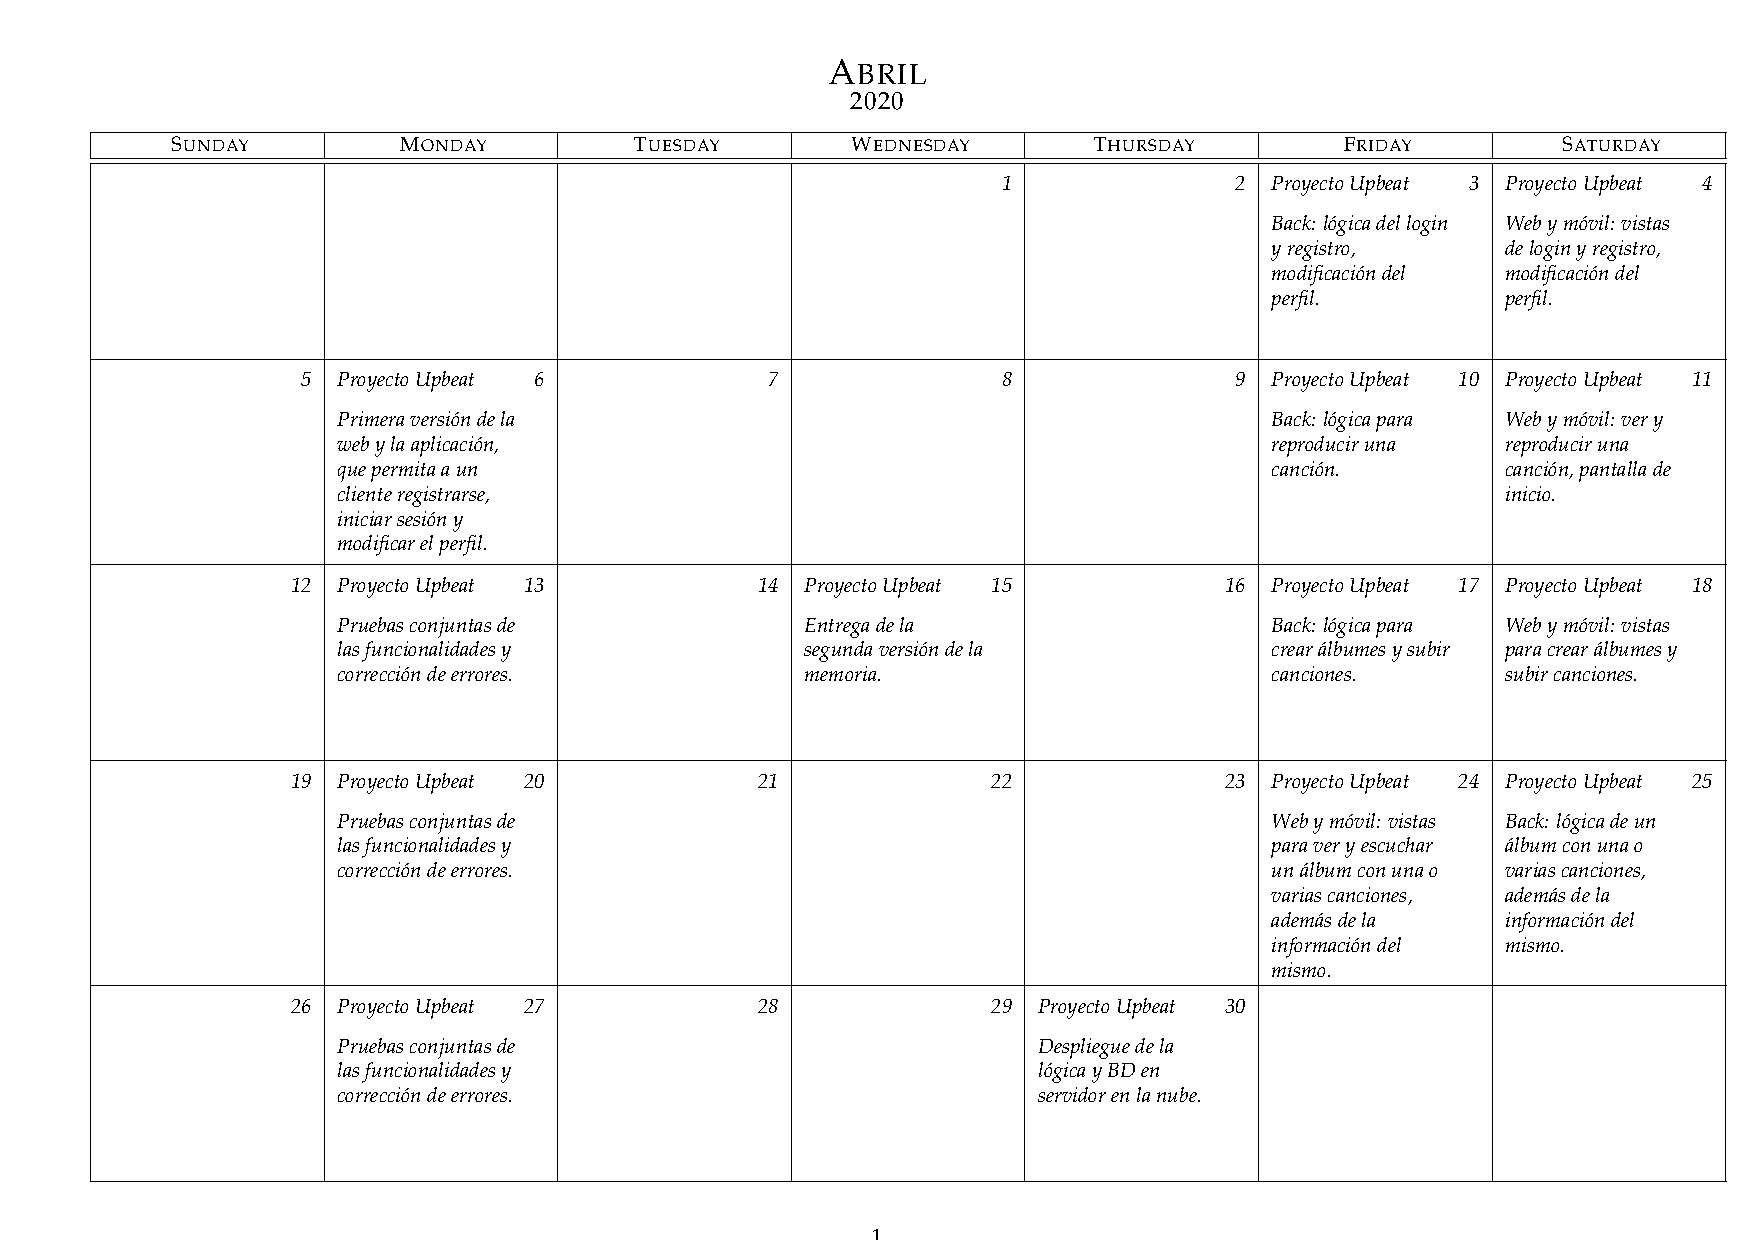
\includepdf[pages=1-2]{calendar.pdf}
\newpage

\subsubsection{Diagramas de Gantt de la aplicación}
\begin{figure}[H]
	\hspace*{-3.7cm}
	\centering{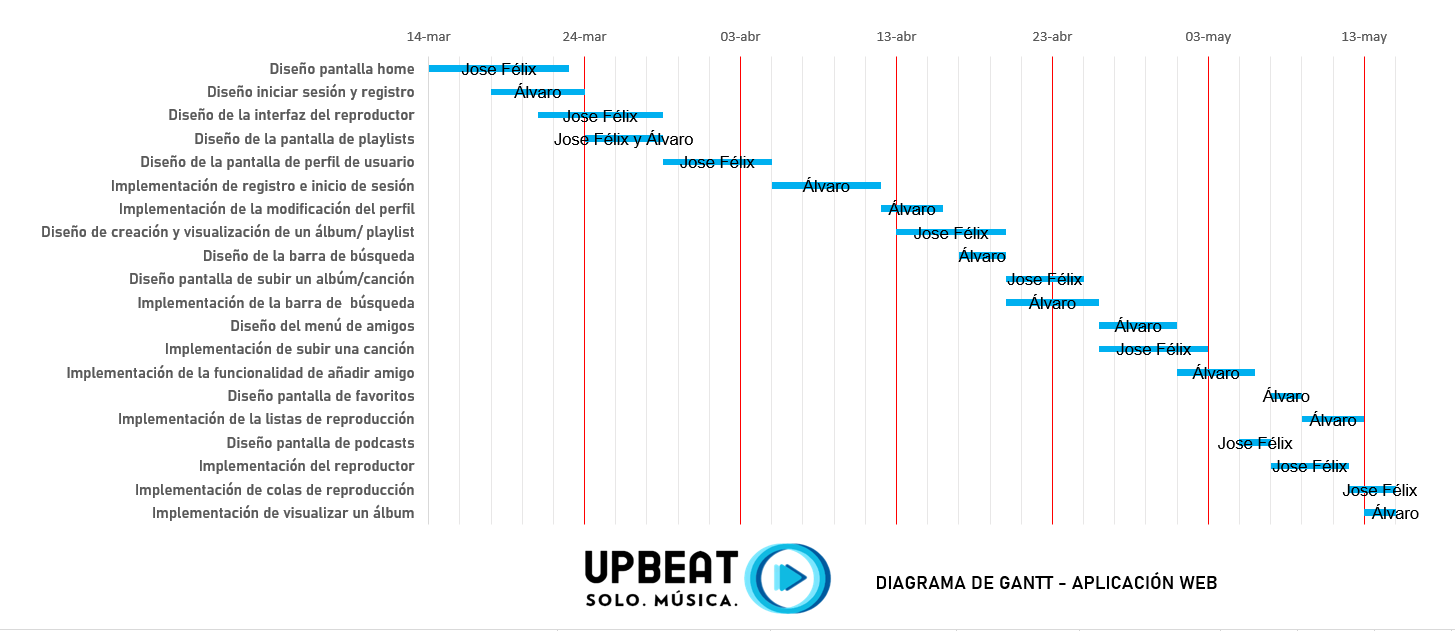
\includegraphics[scale=0.61]{Gantt_app.png}}
\end{figure}
\begin{figure}[H]
	\hspace*{-3.7cm}
	\centering{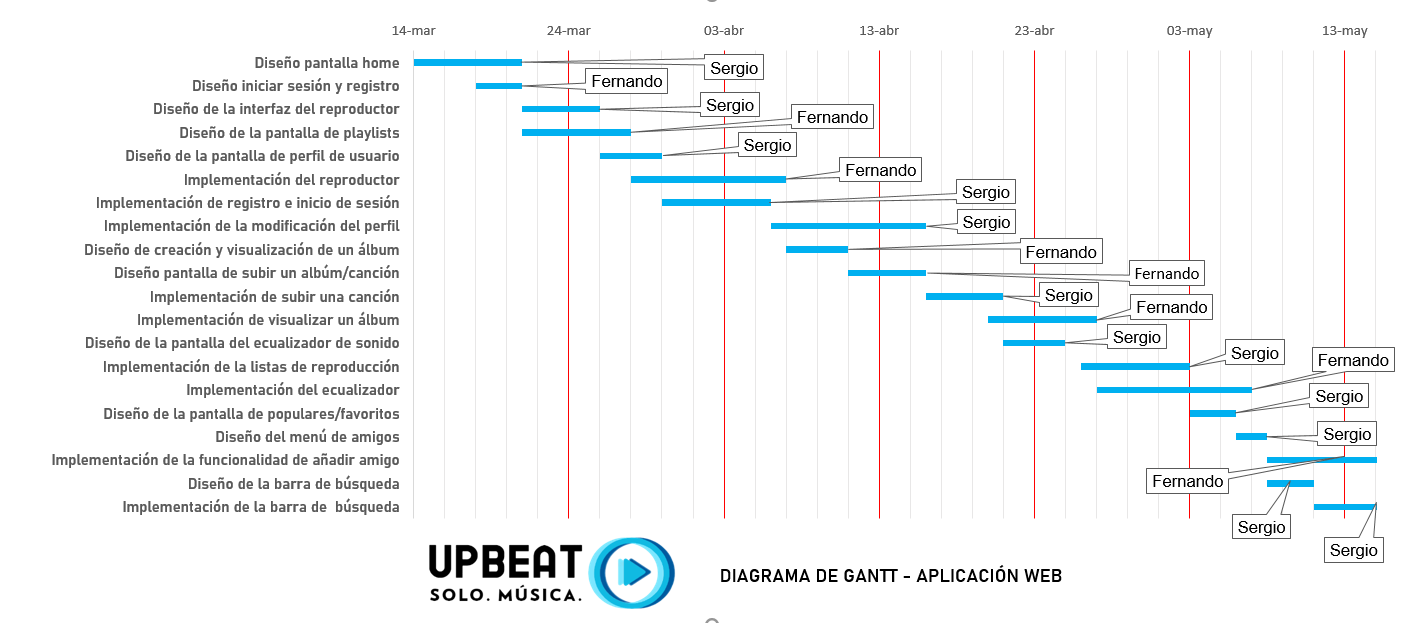
\includegraphics[scale=0.61]{Gantt_web.png}}
\end{figure}
\begin{figure}[H]
	\hspace*{-3.7cm}
	\centering{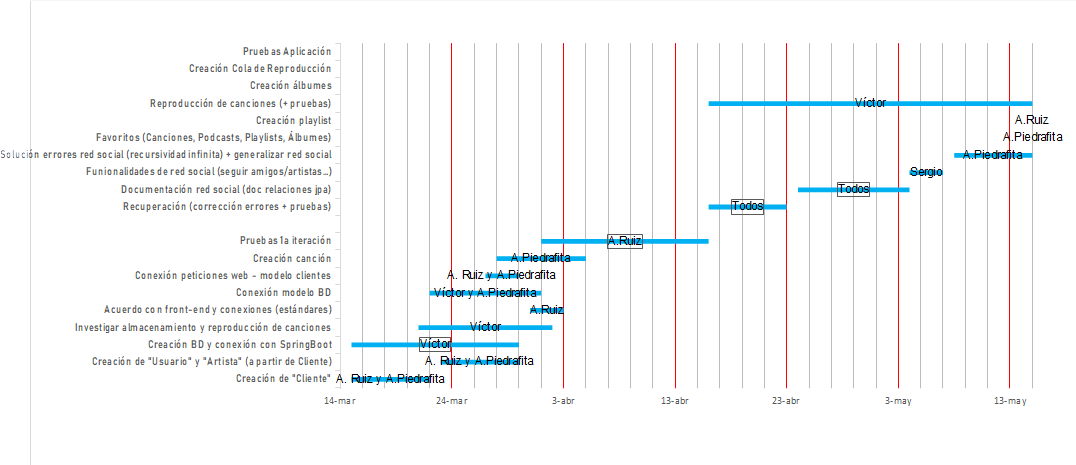
\includegraphics[scale=0.61]{Gantt_back.png}}
\end{figure}

\newpage
\section{Análisis y diseño del sistema}

\subsection{Análisis de requisitos}
Se exponen los siguientes requisitos funcionales de la aplicación:
\begin{table}[H]
	\begin{tabular}{p{4cm} p{10cm}}
		\hline
		\hline 
		\textbf{Requisito funcional}
		\vspace{0.5mm} & \textbf{Descripción} \\ 
		\hline
		\hline
		RF1
		& El sistema permite la existencia de clientes. \\ 
		\hline 
		RF2
		& Los clientes podrán ser usuarios normales o artistas. \\ 
		\hline
		RF3
		& Un cliente se compone de un nombre único, nombre personal y apellidos, un correo electrónico, una contraseña para acceder a la aplicación y una foto de perfil. \\ 
		\hline
		RF4
		& Los clientes accederán al sistema mediante una aplicación móvil o una aplicación web, a través de su correo electrónico y contraseña. \\ 
		\hline
		RF5
		& El sistema permite que los clientes modifiquen los datos de su perfil, es decir, su nombre, correo, contraseña y foto de perfil. \\ 
		\hline
		RF6
		& Un usuario es un cliente registrado que puede acceder a las funciones de la aplicación como escuchar canciones/podcasts, crear y seguir listas de reproducción, seguir a otros usuarios, escuchar álbumes y ver las canciones subidas por los artistas.  \\ 
		\hline
		RF7
		& Un artista es un cliente registrado que puede realizar las mismas funciones que un usuario, además de crear álbumes y subir canciones/podcasts. Solo los artistas puedan subir canciones/podcasts. \\ 
		\hline
		RF8
		&
		Una canción se compone de un título, un audio, artista/s que la han creado, género de la canción, país de la canción y veces que ha sido reproducida.\\
		\hline
		RF9
		&
		Un álbum consiste en la creación de un grupo de canciones que pertenecen al mismo artista. Este posee un título, descripción y una portada.\\
		\hline
		RF10
		& El sistema permite reproducir y pausar una canción y/o podcasts. También permite saltar a la siguiente (si la hubiera), retroceder a la anterior, y elegir un bucle de la misma o reproducir aleatoriamente varias canciones y/o podcasts. \\ 
		\hline
		RF11
		& Una lista de reproducción es una lista de canciones generadas por un cliente. \\ 
		\hline
		RF12
		& El sistema permite que un cliente cree y borre listas de reproducción creadas por ellos mismos, las cuales serán públicas. \\ 
		\hline
		RF13
		& El sistema permite que los clientes añadan o borren canciones a las listas de reproducción creadas por ellos mismos. \\ 
		\hline
		RF14
		& El sistema permite que los clientes sigan listas de reproducción creadas por otros usuarios. \\ 
		\hline
		RF15
		& El sistema permite buscar una determinada canción por nombre o género, además de playlists, artistas y listas de reproducción (esto solo por nombre). \\
		\hline
	\end{tabular}
\end{table}
\break
\begin{table}[H]
	\begin{tabular}{p{4cm} p{10cm}}
		\hline
		\hline 
		\textbf{Requisito funcional}
		\vspace{0.5mm} & \textbf{Descripción} \\ 
		\hline
		\hline
		RF16
		& Las búsquedas por palabras clave deberán al menos contener una palabra, de mínimo cuatro caracteres. \\ 
		\hline 
		RF17
		& El sistema permite ver las canciones más populares de un país. \\ 
		\hline 
		RF18
		& El sistema permite ver las canciones más populares de un artista. \\ 
		\hline
		RF19
		& El sistema permitirá usar un equalizador al escuchar las canciones. \\ 
		\hline
		RF20
		& El sistema permitirá el uso de \textit{banners} para ofrecer publicidad. \\ 
		\hline
	\end{tabular}
\end{table}
Se exponen los siguientes requisitos no funcionales de la aplicación:

\begin{table}[H]
	\begin{tabular}{p{4cm} p{10cm}}
		\hline
		\hline 
		\textbf{Requisito no funcional} & \textbf{Descripción} \\ 
		\hline
		\hline
		RNF1 
		&  El sistema permitirá ser utilizar un diseño modular, un lenguaje fácil de entender, usar y mantener.\\ 
		\hline
		RNF2
		&  El cliente tendrá el desarrollo móvil en formato \textit{Android} e \textit{iOS}.\\ 
		\hline
		RNF3
		& El sistema permite almacenar canciones y podcasts en formato \textit{.mp3}. \\
		\hline
		RNF4
		& El sistema permite las fotos de perfil de los clientes en formato \textit{.png} y \textit{.jpg}. \\
		\hline
	\end{tabular}
\end{table}
\newpage
\subsection{Diseño del sistema}
\subsubsection{Estructura del proyecto}
La estructura global de la aplicación \textit{UPBEAT} será la siguiente:
\begin{figure}[H]
	\hspace*{-1.5cm}
	\centering{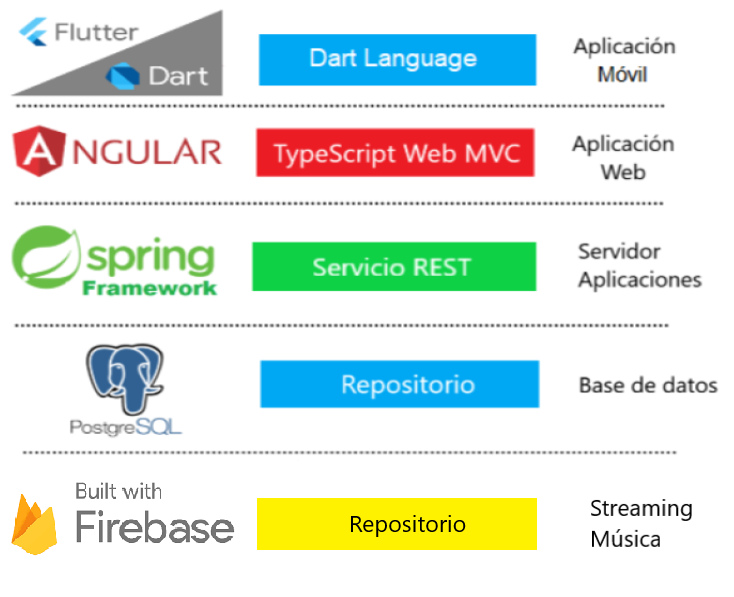
\includegraphics[scale=0.5]{EstructuraProyecto.png}}
\end{figure}
A la izquierda se denotan las tecnologías usadas para cada parte junto a la función que realiza cada una.
\newpage
La manera de comunicarse entre APIs sigue este patrón:
\begin{figure}[H]
	\centering{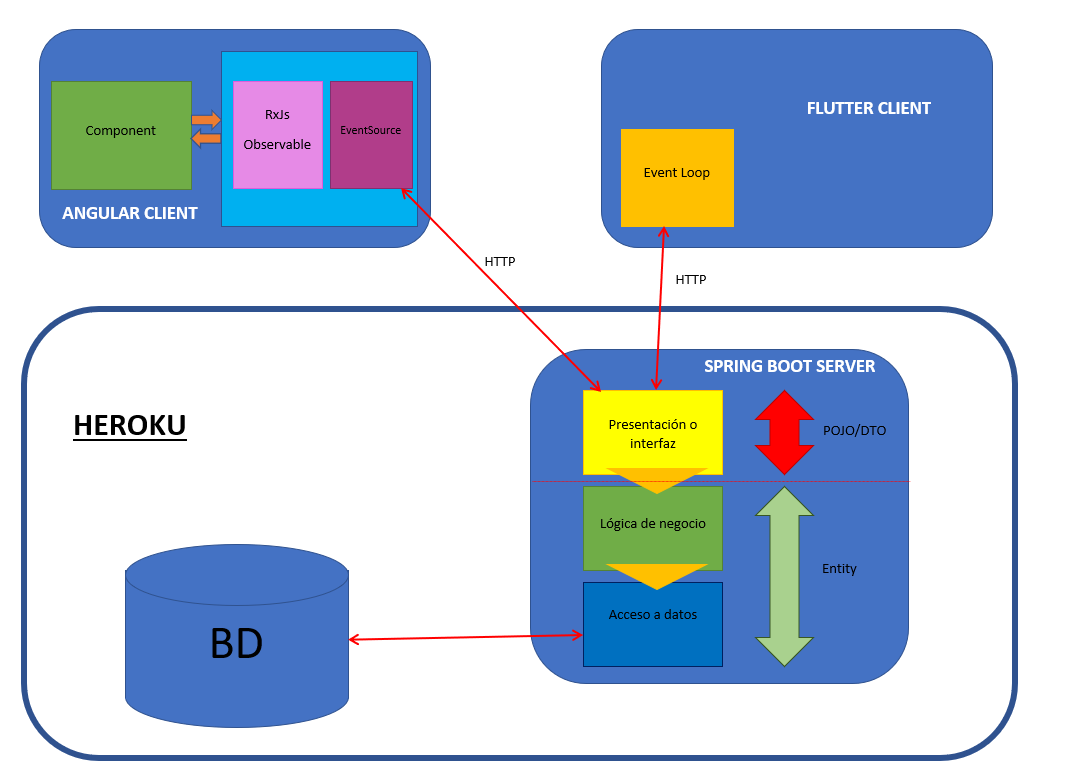
\includegraphics[scale=0.4]{EsquemaPS.png}}
\end{figure}
\subsubsection{Diseño del back-end de la aplicación}
El diseño del back-end será \textit{REST} para todas las consultas y peticiones relacionadas con la aplicación, excepto la parte de las canciones en streaming. Para ello, se usará la tecnología Spring. \\
\hfill \break
Además, también aporta completamente la funcionalidad \textit{CRUD} (\textit{Create == POST}, \textit{Read == GET}, \textit{Update == PUT}, \textit{Delete == DELETE}) en caso de ser necesaria.\\
\hfill \break
Para el desarrollo de streaming, al final se ha optado por la utilización de Firebase como plataforma de guardado y reproducción de los datos.
\subsubsection{Base de datos del proyecto}
Un aspecto esencial que se ha considerado desde el principio ha sido la realización de la base de datos relacional en \textit{PostgreSQL}, siguiendo las siguientes razones:
\begin{itemize}
	\item Brinda opciones más complejas que otros gestores, ya que suele estar orientado para bases de datos más grandes y con consultas más largas. Algunas de sus funciones, como la de unir tablas, hacen que sea mejor valorado por algunos desarrolladores frente a su competencia.
	\item Código \textit{OpenSource}.
	\item Soporta todas las operaciones con \textit{Strings} como concatenar \textit{sub stringing}, búsqueda \textit{regex}, \textit{matching} y \textit{splitting}, búsqueda de texto completo y transformación de caracteres entre otros.
	\item Permite el uso de \textit{JSON} Y \textit{JSONB} en su totalidad, incluyendo varias funciones para el manejo de los mismos.
\end{itemize}
Fue elegido este gestor de datos porque, en comparación con los demás, permite de una manera simple almacenar los datos de las canciones, unido a una alta fiabilidad.
\newpage
El modelo \textit{Entidad - Relación} que se ha llevado a cabo ha sido el planteado a continuación, implementado en el back-end con esta estructura:
\begin{figure}[H]
	\hspace*{-3.9cm}
	\centering{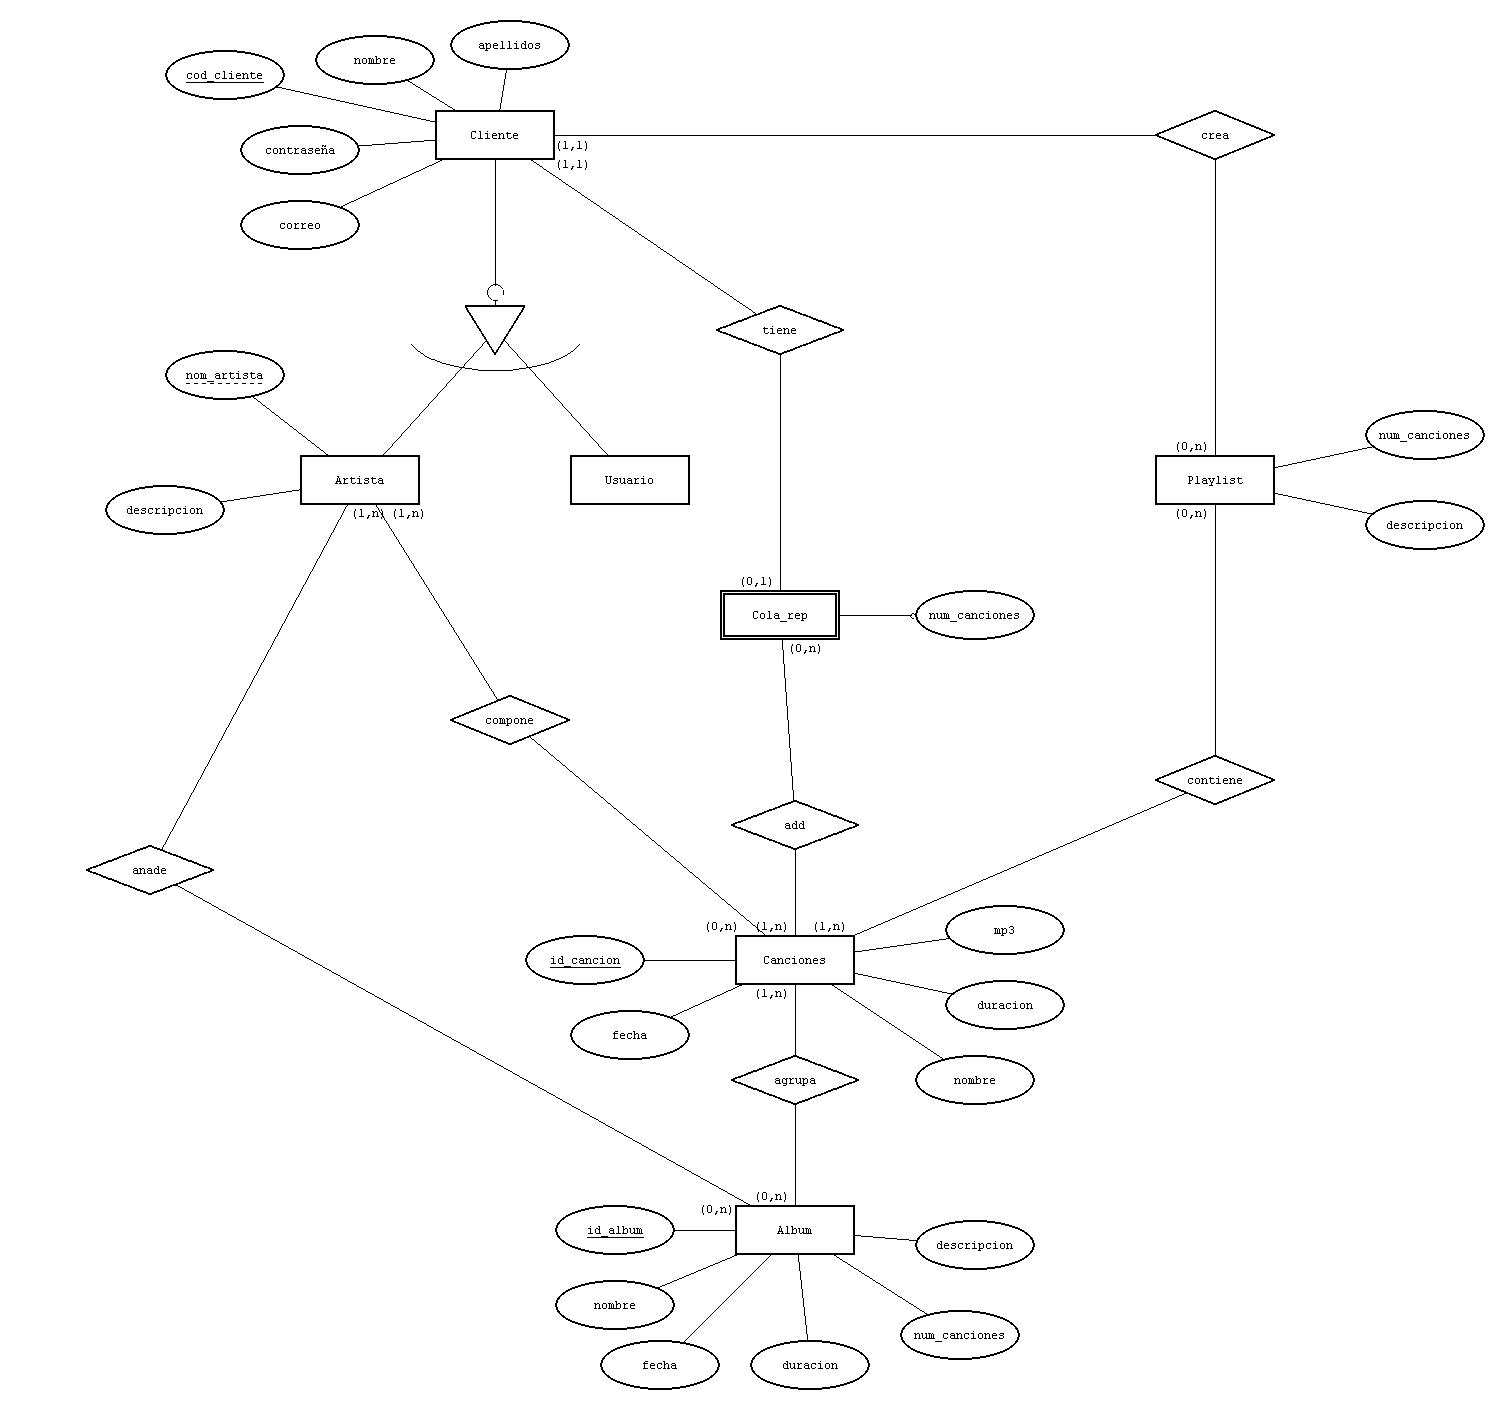
\includegraphics[scale=0.35]{ModeloER.jpg}}
\end{figure}
\newpage
\section{Memoria del proyecto}
\subsection{Inicio del proyecto}
Al principio del proyecto, se creó el documento de propuesta técnica y económica. Este documento está disponible en la carpeta Memoria del \textit{GitHub} del proyecto, donde se explica con más detalle.\\
Una vez creado, se asignaron roles a los distintos integrantes debido a que se trata de un proyecto complejo. Los roles como ya se han mencionado, corresponden con: el jefe del proyecto cuya función principal es la organización, reparto y optimización del trabajo, así como la resolución de posibles disputas en el grupo. 
Se encarga, además, de verificar que todas las tareas sean realizadas a tiempo. \\
\hfill \break
Otro rol sería los responsables de la redacción de las actas, redacción de los documentos no técnicos y por último, los encargados de la redacción de los documentos técnicos y despliegue. Otro rol asignado era la redacción de los guiones de reunión, realizados cada vez que se comunicaba con el profesor. Otros roles, por ejemplo, serán los encargados en la base de datos y servidor, realizando todo el mantenimiento y creación. Similares roles referentes a la aplicación se pueden dividir en 2, los encargados en el diseño de la interfaz web y los encargados en el desarrollo de la interfaz móvil. \\
\hfill \break
El desarrollo del proyecto se realiza a través de la plataforma \textit{GitHub}, de forma que todos los componentes del equipo desarrollan parte del software, y lo ponen en común en dicha plataforma. Se establecieron varias carpetas para cada una de las funcionalidades de la aplicación. \\
Por último, para la elección de las tecnologías usadas, se tuvo principalmente en cuenta los conocimientos del equipo de desarrollo, ya que cuanta mayor experiencia tuviera menos horas aprendiendo dedicarían. Las tecnologías elegidas fueron: bases de datos \textit{SQL}; lenguaje \textit{Dart} para la aplicación móvil; \textit{Angular}, \textit{CSS}, \textit{JavaScript} para web.
\subsection{Ejecución y control del proyecto}
El equipo de \textit{Flutter} ha divido el trabajo asignado a través del diagrama de Gantt correspondiente a móvil. Cada una de las tareas específicas fueron repartidas a un miembro del equipo respectivamente. La comunicación dentro del equipo se ha realizado a través de los mensajes privados de \textit{Whatsapp} ya que solo cuenta con 2 integrantes.\\
Para controlar el trabajo realizado se ha utilizado el \textit{Issue Tracker} de \textit{GitHub}, aunque también nos hemos comunicado por \textit{WhatsApp} para tener una comunicación más activa.\\
\newpage
Se ha ido implementando cada tarea siempre en consonancia con el back-end, por lo que si se producía un retraso en alguna funcionalidad, también implicaba a nuestro desarollo.\\
Al final, los requisitos que no se consiguieron implementar fueron por falta de tiempo o demasiada dificultad con la tecnología escogida.\\
\hfill \break
No se ha producido ningún cambio en las tecnologías empleadas.
No se han producido problemas con las integraciones ni versiones del código.
Las pruebas realizadas han sido comprobar que el front-end se comunica correctamente con el back-end, realizando las consultas e inserciones en la base de datos correctamente.\\
Además, antes de la presentación final se le proporcionó la aplicación a diversas personas del entorno familiar para realizar diversas pruebas (debido a la situación actual de movimiento).\\
\hfill \break
En la parte del front-end web se ha tenido que cambiar la distribución de trabajo, informándonos simultáneamente la mayor parte del tiempo porque no se tenía experiencia previa y había errores de conexión con el back-end que se sabía solventar; todo esto ha llevado mucho tiempo entre leer documentación y realización de pruebas. También cabe reconocer que si se hubiera puesto en contacto antes con los miembros del back-end se habría solventado mucho antes porque eran errores mínimos.\\
\hfill \break
En lo que respecta al back-end, se ha trabajado principalmente por videollamada, trabajando sobre el mismo o diferentes temas, pero cooperando y preguntando dudas en caso de que algún miembro se quede atascado. Previo a esto, han sido necesarias varias horas de formación ya que en la mayoría de los casos no se conocían ni la forma ni el entorno de trabajo. 
Este factor ha hecho que este trabajo haya supuesto un esfuerzo mayor del que podría haber requerido realmente con respecto a las horas.
Además, se ha conseguido desplegar la aplicación en la plataforma \textit{Heroku} para que, cuando se produzca un commit desde la rama master, se suba automáticamente el proyecto y todos los miembros (también desde el front-end) puedan hacer peticiones a las \textit{URLs} previamente acordadas.\\
\hfill \break
Cada equipo encargado de una de las tres partes tenía un calendario propio, que tenían que seguir lo máximo posible siempre y cuando se pudiera.  
Ninguno de los tres grupos acabó dentro de lo establecido por el calendario.\\
\hfill \break
Cada grupo ha intentado seguir esa línea marcada, pero debido a que cada grupo era independiente, afrontaron la compensación del tiempo perdido de distintas maneras.\\
La aplicación móvil sufrió un retraso con respecto al calendario alrededor de 1 ó 2 semanas. Pero se recuperó ese tiempo durante las últimas 2 semanas. Es decir, frente a ese retraso, surgido por problemas de reproducción del streaming. el grupo decidió simplemente hacer jornadas intensivas de desarrollo para alcanzar al calendario.\\
\hfill \break
La página web lleva un retraso respecto al calendario de alrededor de un mes. Los problemas principales por los que ha surgido este retraso son coincidencias de asignaturas, junto con entregas de trabajos, además de la formación en la tecnología. Sin embargo, el motivo principal de que este retraso haya sido mucho más elevado ha sido que no ha habido un ritmo constante en su desarrollo.\\
\hfill \break
El retraso del back-end se debe a la lenta implementación del modelo de streaming. Se tuvo que desechar la idea de usar una tecnología e implementar otra rápidamente que sí dio éxito.
\subsection{Cierre del proyecto}
Como se ha podido ver, la cantidad de horas dedicadas a cada parte ha sido superior a las estimadas, excepto en la parte web, debido fundamentalmente al retraso en el calendario que tenían (lo que hizo que no se pudiera trabajar tanto en ese aspecto). También puede ser debido a una ligera sobreestimación del coste de horas.\\
\hfill \break
Otro punto en el que hay diferencia de horas generalizadas en cada equipo es en el aprendizaje de nuevas tecnologías. Esto es debido a que se estimó que los integrantes tenían un conocimiento muy básico de las herramientas a utilizar y de esa manera se tendría una estimación máxima. Como muchos de los integrantes tenían algún conocimiento previo con las herramientas que utilizaban este coste se redujo.  \\
\hfill \break
Con respecto a la diferencia en esfuerzo, al front-end le ha sido producida por lo recién nombrado y al hecho de que, al no cumplirse el calendario y llevando un gran retraso, como se mencionó en apartados previos, el número de horas es superior al supuesto ya que se dedicó mucho trabajo al final del mismo.\\
\hfill \break
En back-end, las estimaciones propuestas fueron bastante realistas, llegando a ser superior el coste para la implementación mayor que el estimado, aunque el coste en familiarización con las distintas tecnologías fue reducido.\\
\hfill \break 
Las estimaciones para la aplicación móvil no sufrieron grandes cambios. Como ya se ha dicho se hizo una estimación alta para el diseño de la interfaz, mientras que el coste de su implementación iba a ser relativamente bajo. \\
Pero debido a que se hizo una aplicación nativa el coste de su producción se incrementó. La diferencia entre el coste estimado y el real es muy bajo, por lo que la estimación que se hizo fue bastante ajustada a la realidad. \\
\hfill \break
También se hizo una estimación de las pruebas que no se pudo cumplir del todo, ya que debido a los retrasos producidos en la aparte web y ligeramente en Android, hizo que no se puedan realizar todas las pruebas esperadas. Con lo cual la cantidad de esfuerzo dedicado a las pruebas es menor.\\
Como ya se ha dicho anteriormente, había gente que no controlaba demasiado las tecnologías utilizadas, así que el hecho de participar en este proyecto ha hecho que todos los integrantes puedan aprender algo más acerca de distintas tecnologías. \\
\hfill \break
En primer lugar, GitHub. Muy pocos de los integrantes habían utilizado esta clase de herramienta, lo que ha permitido que este proyecto haya sido útil para aprender esta herramienta ya que, de no haberla utilizado, hubiera sido muy complicado la división del trabajo y la unión de todo lo realizado por cada integrante. El hecho de haber aprendido a utilizar esta herramienta es útil ya que, en el futuro, al intentar hacer cualquier proyecto de tamaño medio-grande sería necesaria esta herramienta, por lo que esa experiencia ya se ha obtenido.\\
\hfill \break
Ciertas personas no habían aprendido ciertas tecnologías del back-end o front-end, pero por distintos motivos han participado en ese equipo, lo que ha hecho que hayan tenido que aprender las tecnologías correspondientes desde prácticamente el principio. Esto hace que si en algún momento tienen que participar en algún proyecto en el que necesiten eso ya tendrán un conocimiento lo suficientemente alto de esa tecnología como para desenvolverse relativamente bien. \\
\hfill \break
Puesto que al final se decidió hacer la versión para Flutter nativa, la gente que no hubiera estado en contacto con esta tecnología también pudo aprender a utilizar este entorno para la creación de aplicaciones móviles.\\
\hfill \break
Las horas trabajadas se han contabilizado en el Anexo II del proyecto.
\newpage
\section{Conclusiones}
\subsection*{Alejandro Piedrafita}
En esta asignatura, se ha realizado un proyecto software el cual ha supuesto planear y más tarde llevar a cabo todas y cada una de las fases que implica un proyecto de este estilo. Durante la realización de este proyecto y, sobre todo, con el transcurso de los días, se han debido de afrontar diversos retos y complicaciones, tanto planeados como imprevistos. A pesar de ello, se ha conseguido finalmente sacar adelante dicho proyecto y poder presentar una aplicación de streaming de música funcional para ordenador y sobre todo para móvil.\\
\hfill \break
La primera de las complicaciones ha sido familiarizarse con el entorno de trabajo, las configuraciones y demás aspectos específicos del entorno. Tanto a nivel de grupo como a nivel personal, esto supuso un gran periodo de adaptación. Personalmente me implicó más tiempo del planeado el familiarizarme con la forma de trabajar, crear y gestionar proyectos, pero es algo que debe hacerse para poder posteriormente trabajar de forma autónoma y avanzar en el proyecto.\\
\hfill \break
Otro de los aspectos clave que se han podido observar a lo largo del proyecto es la definición de roles inicial, así como las tareas asignadas a cada individuo. Este es un aspecto fundamental, el cual debe quedar claro desde un inicio y respetarse durante todo el proyecto. Cada individuo debe conocer sus virtudes y sus debilidades y ser realista a la hora de definir dichos roles y tareas, pues de lo contrario esto supone un coste extra de trabajo y estrés para el resto del grupo teniendo que asumir dichas tareas si se quiere sacar el proyecto adelante.\\
\hfill \break
Un aspecto muy importante a destacar, definido en la asignatura pero no siempre llevado a la práctica, es el control de esfuerzos. De esta forma se puede llevar al día qué se ha realizado y qué queda aún por realizar, tener en cuenta los imprevistos y pedir ayuda en caso de ser necesitada. Es importante seguir un orden lógico y únicamente dar por terminadas las tareas cuando han sido completadas y probadas, pues de lo contrario perjudica tanto al propio grupo como al resto de grupos sin poder continuar y generando dudas. Para complementar este aspecto, ha resultado de gran utilidad el control de versiones y líneas de código de cada miembro, permitiendo así identificar quién ha añadido cada línea, en qué momento y en qué archivo. Esto permite identificar de forma mucho más rápida y clara los nuevos cambios (verde, amarillo y rojo) pudiendo así comprender el código de los compañeros en cada fecha.\\
\hfill \break
Sí cabe destacar como punto fuerte y muy positivo la comunicación entre grupos, coordinándose e informando de sus avances y sus limitaciones. Muchas de las pruebas se realizaron en conjunto, cooperando varios grupos al mismo tiempo. Se debe destacar la predisposición a ayudar de los miembros de la aplicación móvil, tanto para las pruebas conjuntas como incluso para ayudar en aspectos de código y configuración a nuestro grupo (back-end).
\subsection*{Sergio Torres}
Las conclusiones que puedo sacar de este proyecto son, principalmente, lo difícil que puede llegar a ser tener un producto final de calidad sin una buena planificación y lo importante y complicado que es tener una idea realista de lo que quieres que tenga la aplicación final desde un punto inicial del proyecto.\\
\hfill \break
La planificación en mi opinión podría haber sido mejor, esto es porque desde el inicio se desconocía bastante el coste de lo que nos iba a suponer la implementación de todos los requisitos y funciones que queríamos que tuviera nuestra aplicación. A esto le sumo una planificación demasiado flexible con las tareas que nos asignábamos. Creo que es bueno que tenga un punto de flexibilidad, pero ya hemos visto que si se excede ese punto da lugar a una organización más complicada.\\
\hfill \break
En cuanto a los requisitos funcionales, se ha comprobado que son fáciles de definir pero difíciles de implementar, sobre todo si no se tiene un conocimiento suficiente ni experiencia previa sobre las herramientas de desarrollo utilizadas (Angular, en mi caso) y con los lenguajes de programación utilizados (TypeScript, principalmente). Es por ello por lo que el inicio del proyecto se hace duro en estas ocasiones.\\
\hfill \break
Finalmente, estoy contento con lo aprendido ya que, además de haber cogido soltura en el manejo de estas nuevas herramientas de desarrollo web y sus lenguajes de programación, haciendo un proyecto de esta magnitud es cuando te das cuenta de la importancia de tener una buena planificación y unos requisitos funcionales que puedas llevar a la práctica a tiempo.\\
\hfill \break
Considero que es necesario tener en cuenta los errores, admitirlos y analizarlos como se ha hecho en este apartado de conclusiones para poder mejorar en el futuro, ya que todo se simplifica a eso.
\newpage
\subsection*{Víctor Pérez}
La principal conclusión que he sacado tras la realización de este trabajo es que, durante un proyecto largo viene bien dividir el trabajo en tareas más pequeñas y que, aunque a veces algunas de esas tareas se alarguen más de lo que se esperaba hay que saber reorganizar el tiempo sobre la marcha. \\
\hfill \break
Siguiendo con el punto anterior se podría haber mejorado un poco la parte concerniente al seguimiento del calendario, por mi parte sobre todo me costó bastante más de lo habitual la parte del streaming de canciones. Quizás por empeñarme en realizarlo de la forma en la que se había planeado en un principio en vez de abrirme a cambiar la manera de hacerlo antes, lo que, visto a posteriori, habría ahorrado bastante tiempo y ajustado el calendario, ya que bastantes funcionalidades y pruebas dependían de ello.\\
\hfill \break
Por otra parte, si que es verdad que ha sido de los pocos proyectos de tanta extensión que hemos realizado en la carrera, y la verdad que seguir la metodología de trabajo que hemos decidido, tanto en división de tareas como en el control de versiones etc, nos ha ayudado a no tener que preocuparnos por demasiados conflictos en los merges de github y han facilitado el trabajo en equipo.\\
\hfill \break
Respecto a los conocimientos aprendidos, en esta práctica he adquirido bastantes conocimientos sobre el tema de aplicaciones web y rest API ya que, aunque el lenguaje de java que se ha usado en el back era conocido para mí, nunca lo había usado en estos términos, además me gustaría incluir en esta parte también la metodología de trabajo mencionada en el párrafo anterior ya que considero que me puede ser de gran utilidad en un futuro.
\subsection*{Álvaro Santamaría}
En esta asignatura hemos afrontado y superado el reto de desarrollar un proyecto de software de una manera muy similar a cómo lo haremos en el futuro en una empresa, trabajando con tecnologías nuevas y desconocidas hasta ahora y enfrentándonos a los problemas de una forma más autónoma e independiente con respecto a proyectos y trabajos grupales previos de otras asignaturas en la titulación.\\
\hfill \break
En mi caso particular, lo más importante que he aprendido es que el resultado final depende de una correcta y continua organización. Mi apreciación es que nuestro grupo no estuvo lo suficientemente organizado como para cumplir los plazos que se habían propuesto en un inicio y que, viendo como el tiempo se nos echaba encima, en lugar de pararnos y reestructurar todo, se optó por realizar sesiones exhaustivas de trabajo de forma independiente para poder llegar a tener una aplicación mínimamente funcional, lo cual supuso que se aumentaran considerablemente las horas de trabajado que en un principio habían sido establecidas.\\
\hfill \break
Además, creo que también ha faltado coordinación entre los diferentes equipos de desarrollo ya que en varias situaciones se habrían subsanado muchos errores que surgían si hubiésemos preguntado al resto de equipos en lugar de intentarlos resolver de forma autónoma.\\
\hfill \break
En mi opinión, nadie ejerció de líder de tal forma que nos coordinásemos todos los desarrolladores del proyecto en lugar de cada equipo fuese por libre. También echo en falta un mayor número de sesiones de control para poder saber cuál era la situación en la que se encontraban el resto de equipos de trabajo.\\
\hfill \break
Cabe destacar que no todo ha sido negativo, puesto que hemos sido capaces de aprender un nuevo lenguaje de programación (en mi caso el lenguaje Dart) y ser capaces de desarrollar una aplicación móvil totalmente funcional en este cuatrimestre cumpliendo con la mayoría de los requisitos prestablecidos, pese a todos los inconvenientes y problemas previamente citados.\\
\hfill \break
Por último destacar también la buena comunicación que hubo en mi equipo de desarrollo de frontend móvil formado por José Félix y por mí, ya que en todo momento nos hemos ayudado mutuamente para conseguir los objetivos.
\subsection*{José Félix Yagüe}
En esta asignatura he aprendido la importancia de la planificación en un proyecto de gran escala, y la importancia de utilizarla correctamente y seguirla día a día, ya que es una herramienta muy útil de la que no era realmente consciente hasta el momento.\\
\hfill \break
Al estar tanta gente trabajando en un mismo proyecto utilizarla nos ha hecho la vida bastante más fácil a la hora de hacer funcionar todo correctamente.
También he visto la importancia de trabajar en equipo porque al ser un trabajo tan grande del que dependes de lo que ha desarrollado otra persona para poder trabajar en tu parte. Te das cuenta de lo que importa trabajar con otras personas para poder hacer funcionar trabajos más complejos que los que habíamos hecho hasta ahora.\\
\hfill \break
Si tuviese que hacer algún cambio respecto a lo que hemos hecho sería sobretodo seguir mejor la planificación que se había desarrollado al principio, ya que hemos tenidos retrasos acumulados desde casí el inicio del proyecto. Estos retrasos son más grandes en trabajos de este tipo donde muchas veces el trabajo de unos depende de otros.\\
\hfill \break
Dicho esto creo que la planificación que habiamos hecho estaba bien planteada, por lo que la haría de la misma forma si tuviesemos que hacer otro proyecto así.
\newpage
Por último, recalcar que a pesar de los retrasos, que ha sido el único aspecto negativo, me ha parecido una buena experiencia que podemos usar para aprender de los errores y no volver a caer en ellos en proyectos futuros de gran escala.
\subsection*{Fernando Navarro}
Las conclusiones que saco de este proyecto es que tener una buena planificación es la gran parte del proyecto porque aunque dispongas de gente que dedique muchas horas y mucho esfuerzo si no hay una buena planificación prácticamente no sirve de nada. En nuestro proyecto hemos sido un poco laxos y permisivos en cuanto a ir modificando la planificación sobre la marcha y dejar tareas sin completar que se acumulaban semanas más tarde.\\
\hfill \break
Por mi parte creo que el principal error fue no calcular bien el tiempo que me iba a costar aprender a usar Angular y los lenguajes que utilizaba. Respecto al proyecto en general el error más grave fue elegir mal el almacenamiento de las canciones y los podcasts que fue lo que retrasó la mayor parte del proyecto. Por eso si ahora volviésemos a empezar el proyecto empezaríamos cambiando esas elecciones además de hacer una planificación más estricta a la que todo el mundo estuviese sujeto y seguro que se habrían podido implementar todos los requisitos funcionales, teniendo un producto final mucho mejor.\\
\hfill \break
A pesar de todo esto creo que he aprendido bastante de esta asignatura porque he hecho mucho autoaprendizaje de cosas que no había hecho hasta ahora y también he aprendido de lo que hemos hecho mal. Creo que es difícil que algo salga a la perfección la primera vez que lo haces y era el caso de este primer proyecto.
\subsection*{Alejandro Ruiz}
De este proyecto, y sobretodo del resultado obtenido (producto resultante), se puede concluir que un buen producto empieza por una buena gestión. Esta conclusión se ve clara al darnos cuenta de que nuestra mejorable gestión ha dado lugar a un producto bueno, pero no excelente. \\
\hfill \break
Centrándonos en la gestión como tal, si tuviésemos que iniciar un nuevo proyecto, aplicando los conocimientos adquiridos de esta experiencia, lo primero que haría sería aclarar desde un comienzo los papeles de cada trabajador y establecer una jerarquía clara (lo cual si hicimos), y establecería unos procesos de control y medidas de avance del proyecto lo más concretos posibles (lo cual no hicimos bien), para intentar seguir el calendario paulatinamente. \\
\hfill \break
En general, aplicaría una metodología de procesos mucho más metódica, ya que la que hemos llevado acabo ha dejado algunas cosas sin terminar. 
Y diría que uno de los mayores problemas, ha sido la indulgencia generalizada, en la que pese a ir retrasados, se iba perdonando y diciendo el “ya lo recuperarás”. \\
En un ambiente laboral, esto sería sin duda lo primero que se solventaría al jugarse el sueldo, ya que aquí al no haber dicho riesgo, nadie sentía ese nivel de responsabilidad. \\
\hfill \break
Sin embargo, resulta interesante realizar un proyecto de estas características debido a su aproximación con un futuro laboral, ya que en cualquier trabajo se tiene que coordinar en grupo. \\
En este sentido ha sido de gran utilidad, y además en el uso de herramientas comerciales que puede utilizar cualquier empresa destinada al desarrollo software. \\
\hfill \break
Además, el conocimiento sobre nuevas tecnologías y su reflejo en una aplicación real han sido otros factores positivos del trabajo.
\newpage
\section*{Anexo I. Actas de las reuniones}
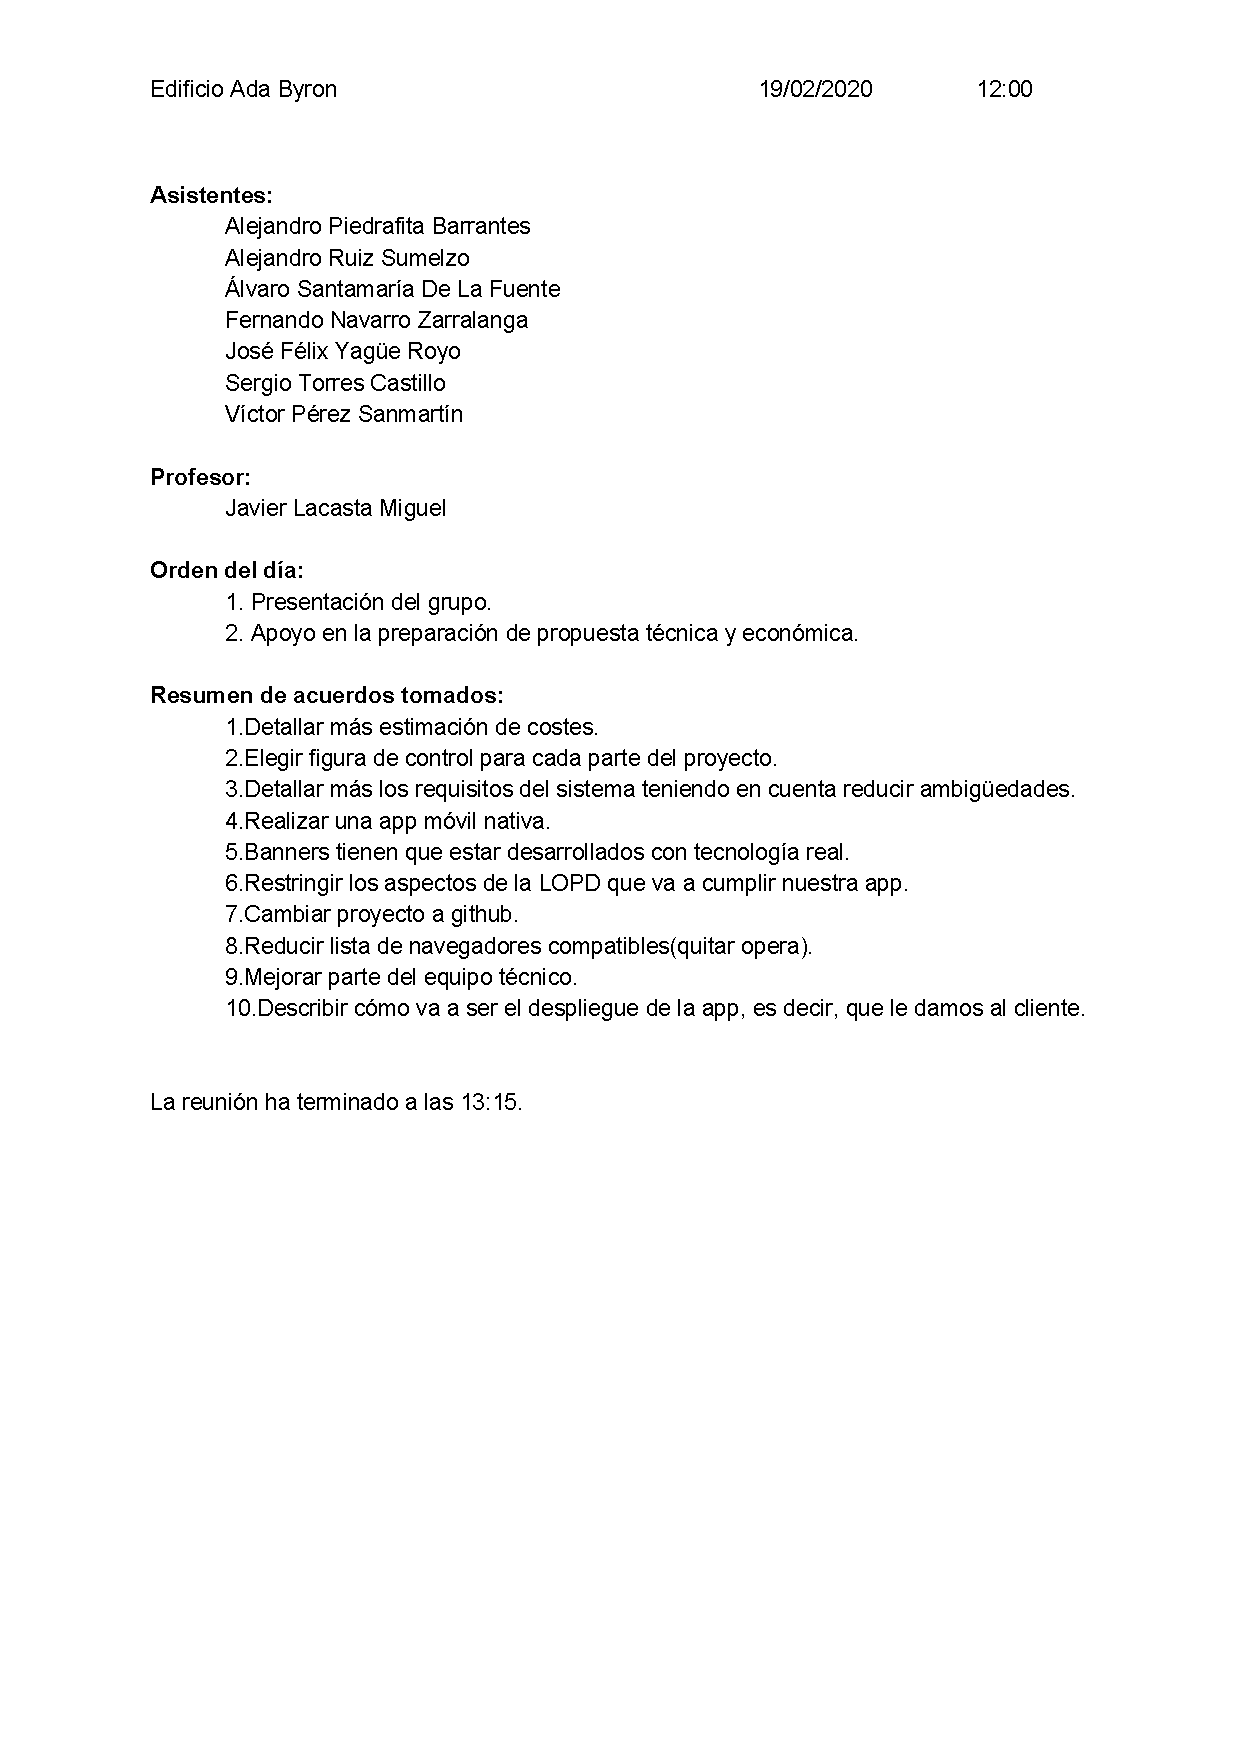
\includepdf[pages=1-5]{actas.pdf}
\newpage
\section*{Anexo II. Esfuerzos realizados}
\begin{table}[H]
	\centering
	\resizebox{\textwidth}{!}{%
		\begin{tabular}{|c|c|c|}
			\hline
			\multicolumn{1}{|l|}{\textbf{Miembro del equipo}} &
			\multicolumn{1}{l|}{\textbf{Horas dedicadas}} &
			\textbf{Tarea} \\ \hline
			\textbf{Alejandro Ruiz} &
			120 h &
			\begin{tabular}[c]{@{}c@{}}Responsable del equipo\\ Coordinador de la memoria\\ Desarollo del back-end\end{tabular} \\ \hline
			\textbf{Álvaro Santamaría}    & 130 h & Desarrollo del front-end     \\ \hline
			\textbf{José Félix Yagüe}     & 120 h & Desarrollo del front-end     \\ \hline
			\textbf{Alejandro Piedrafita} & 145 h & Desarrollo del back-end      \\ \hline
			\textbf{Víctor Pérez}         & 105 h & Desarrollo del back-end      \\ \hline
			\textbf{Sergio Torres}        & 135 h & Desarollo del front-end web  \\ \hline
			\textbf{Fernando Navarro}     & 100 h & Desarrollo del front-end web \\ \hline
			\textbf{Total}                & 855 h & \multicolumn{1}{l|}{}       \\ \hline
		\end{tabular}%
	}
\end{table}
\newpage
\section*{Anexo III. Propuesta técnica y económica}
\begin{figure}[H]
	\centering{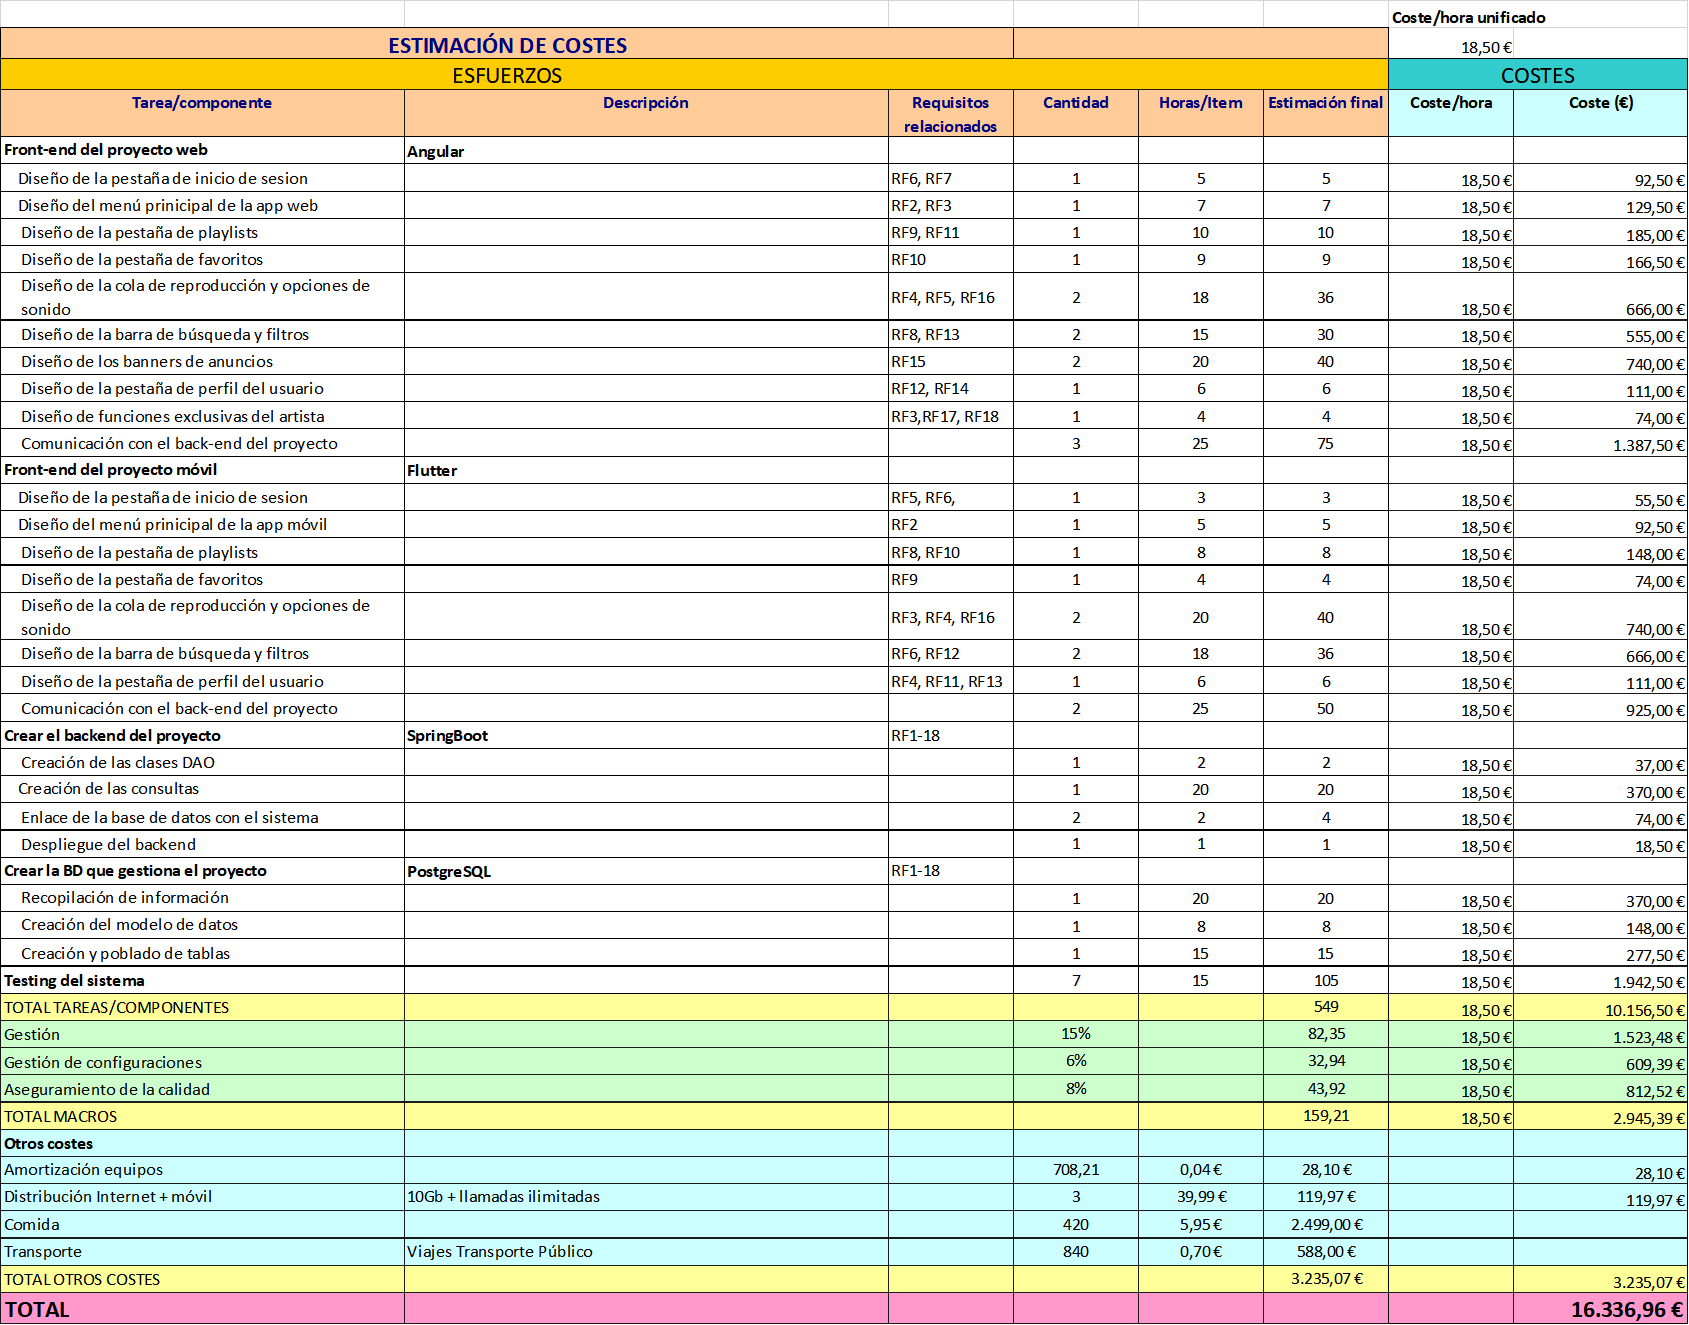
\includegraphics[scale=0.35]{EstimacionCoste.png}}
\end{figure}
\end{document}


